\documentclass[10pt,letterpaper]{article}
\usepackage[top=1in,bottom=1in,left=1in,right=1in]{geometry}
\usepackage{datetime}
\usepackage{natbib}      % http://merkel.zoneo.net/Latex/natbib.php
\usepackage{palatino}
\usepackage{verbatim}
\usepackage[normalem]{ulem}
\bibpunct{(}{)}{;}{a}{,}{,}

\usepackage{array}

\usepackage{chngpage}
\usepackage{stmaryrd}
\usepackage{amssymb}
\usepackage{amsmath}
\usepackage{graphicx}
\usepackage{lscape}
\usepackage{subfigure}
\usepackage[usenames,dvipsnames]{color}
\definecolor{myblue}{rgb}{0,0.1,0.6}
\definecolor{mygreen}{rgb}{0,0.3,0.1}
\usepackage[colorlinks=true,linkcolor=black,citecolor=mygreen,urlcolor=myblue]{hyperref}

\newcommand{\bocomment}[1]{\textcolor{Bittersweet}{BO says: #1}}

\newcommand{\ignore}[1]{}
\newcommand{\transpose}{^\mathsf{T}}
\newcommand{\inner}[1]{\langle #1 \rangle} 
\newcommand{\smallsec}[1]{\noindent \textbf{#1\ }}
\newcommand{\cmd}[1] {{\color{blue}\texttt{#1}}}

\newcommand{\solution}[1]{{\color{myblue} \emph{[Solution:} 

#1 

\emph{End solution]}}}
\newcommand{\solutionnote}[1]{{\color{myblue} \emph{[Note:}

#1 

\emph{End note]}}}
\newcommand{\points}[1]{{\color{mygreen}\emph{[#1]\ \ }}}

\newcommand{\aone}{\diamondsuit}
\newcommand{\atwo}{\heartsuit}
\newcommand{\bone}{\triangle}
\newcommand{\btwo}{\Box}
\newcommand{\myand}{\ \land\ }
\newcommand{\myor}{\ \lor\ }
\newcommand{\mynot}{\lnot}

\title{
  \textbf{Mini-project 4: Recognition} \\
  \Large{CMPSCI 670, Fall 2016, UMass Amherst} \\
  \Large{Due:  November 28, 5:00 PM } \\
  \Large{Instructor: Subhransu Maji} \\
  \Large{TA: Tsung-Yu Lin}
}


\settimeformat{ampmtime}
\date{}
\begin{document}
\maketitle

\renewcommand\thesubsection{\thesection.\alph{subsection}}


\section*{Guidelines}

\paragraph{Submission.} Submit a \emph{single pdf document} via moodle that includes your solutions, figures and printouts of code. For readability you may attach the code printouts at the end of the solutions. You could have 24 hours late submission with a 50\% mark down. Late submission beyond 24 hours will not be given \emph{any} credits. 

\paragraph{Plagiarism.} We might reuse problem set questions from previous years, covered by papers and webpages, we expect the students not to copy, refer to, or look at the solutions in preparing their answers. We expect students to want to learn and not google for answers. 

\paragraph{Collaboration.} The homework must be done individually, except where otherwise noted in the assignments. 'Individually' means each student must hand in their own answers, and each student must write their own code in the programming part of the assignment. It is acceptable, however, for students to collaborate in figuring out answers and helping each other solve the problems. We will be assuming that you will be taking the responsibility to make sure you personally understand the solution to any work arising from such a collaboration.

\paragraph{Using other programming languages.} All of the starter code is in Matlab which is what we expect you to use. You are free to use other languages such as Octave or Python with the caveat that we won't be able to answer or debug non Matlab questions.



\newpage

\section*{The MNIST dataset}
In this homework you will implement several image features and evaluate their performance using logistic-regression classifiers on three variants of the MNIST digits dataset:
\begin{itemize}
\item \textbf{normal} -- the standard MNIST dataset (File \cmd{digits-normal.mat})
\item \textbf{scaled} -- where the pixel values of each image in the normal dataset are replaced as $I \leftarrow a*I + b$ where $a$ and $b$ are random numbers $\in [0,1]$ (File \cmd{digits-scaled.mat}). 
\item \textbf{jittered} -- where the image is translated within each image randomly between $[-10,10]$ pixels both in the horizontal and vertical directions (File \cmd{digits-jittered.mat}).
\end{itemize}

The ``normal" dataset can be loaded into Matlab by typing $\cmd{load(../data/digits-normal.mat)}$. This loads a structure called \cmd{data} which has the images, labels and the splits in variables \cmd{x}, \cmd{y}, and \cmd{set} respectively. E.g., $\cmd{data.x}$ is an array of size $28 \times 28 \times 1 \times2000$ containing $2000$ digits. Class labels are given by the variable $\cmd{data.y} \in \{0,1,\ldots, 9\}$. Thus, pixel \cmd{(i,j)} in the the \cmd{k'th} training example is \cmd{data.x(i,j,1,k)} with label \cmd{data.y(k)}. The \cmd{data.set} has values $\in\{1,2,3\}$ corresponding to train, val, and test splits respectively.

\begin{figure}[h]
\centering
\begin{tabular}{ccc}
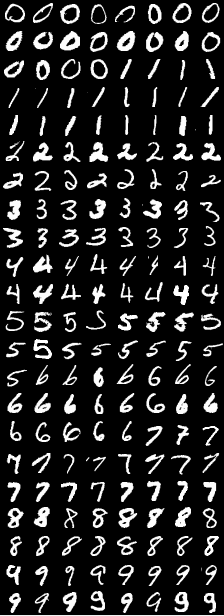
\includegraphics[width=0.28\linewidth]{digits-normal.png} & 
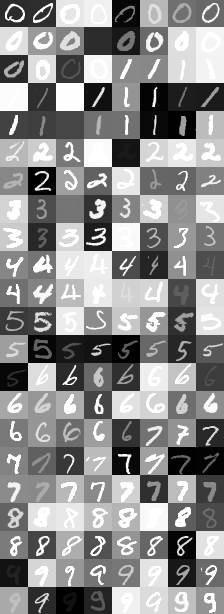
\includegraphics[width=0.28\linewidth]{digits-scaled.png} & 
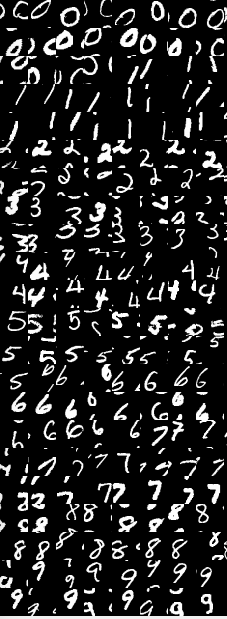
\includegraphics[width=0.28\linewidth]{digits-jittered.png} \\
(a) normal & (b) scaled & (c) jittered \\
\end{tabular}
\caption{Example images from different variants of the MNIST dataset. You can visualize the images using $\cmd{montageDigits}$ function included in the codebase.} 
\end{figure}







\newpage

\section{Image representations}

Implement three different image representations described below. 

\subsection{Pixel features}
Implement the function \cmd{features = extractDigitFeatures(x, 'pixel')} that takes as input the images \cmd{x} and returns their pixel values as a feature. You have to simply reshape the $28\times28$ pixel image into a vector of size $784\times 1$. The variable \cmd{features} is a array of size $784\times N$ where $N$ is the number of images in \cmd{x}. 

\subsection{Histogram of oriented gradients}
Implement the function \cmd{features = extractDigitFeatures(x, 'hog')} that takes as input the images \cmd{x} and returns their histogram of oriented gradients (HoG) as a feature. Recall the steps in the HOG feature computation are:
\begin{enumerate}
\item Apply non-linear mapping to input image
\item Compute horizontal and vertical gradients gx and gy at each pixel using derivative operators. Compute the magnitude $m = \sqrt{gx^2 + gy^2}$ and orientation $\theta=\arctan(gy/gx)$ at each pixel. 
\item Given a spatial binSize and number of orientation bins (numOri) define a grid of binSize$\times$ binSize across the image and compute the orientation histogram weighted by gradient magnitudes within each grid cell by quantizing the orientation into numOri bins. Concatenate these histograms to obtain an image representation.
\item Local and global normalization steps.
\end{enumerate}

To begin with you can ignore initial non-linear mapping (Step 1) and local normalization (part of Step 4). You will investigate the effect of global normalization in the next section.

\subsection{Local binary patterns}
Implement the function \cmd{features = extractDigitFeatures(x, 'lbp')} that takes as input the images \cmd{x} and returns a local binary pattern (LBP) histogram for each image. Local binary patterns are a class of highly effective feature representations.


You will implement a simplifed version that maps each 3x3 patch into a number between 0 and 255 as follows. Consider the pixel values in the 3x3 patch. Subtract from each pixel the value at the center. Compute the sign of resulting value at each of the 8 positions (exclude the center). This gives us a 8 bit number which the representation of the 3x3 patch. The scheme is shown in the Figure below.

You can apply this scheme to each pixel in the image (excluding the border) and obtain a number between 0 and 255 for it. The overall LBP histogram is obtained by counting how many times each value appears in the image.  

\begin{figure}[h]
\centering
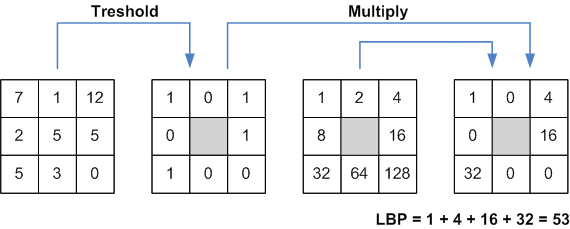
\includegraphics[width=0.5\linewidth]{lbp.png}
\caption{Illustration of the LBP feature computation for a 3x3 patch.} 
\end{figure}

\section{Normalization}
After you implement these features you may find that the scales of the features can vary  dramatically on some datasets for some features. For example, on the ``scaled" version of the digits the raw pixel values are randomly perturbed making the pixel representation less robust. Implement the following steps:
\begin{enumerate}
\item \textbf{Square-root scaling} -- replace the value of each feature by its square-root, i.e., $x \leftarrow \sqrt{x}$.

\item \textbf{L2-normalization} -- scale each feature vector to unit length, i.e., if $\mathbf{x}$ is a vector then the L2-normalized version would be $\mathbf{x} \leftarrow \mathbf{x}/\sqrt{\sum_i \mathbf{x}_i^2}$
\end{enumerate}

The effectiveness of one or both of these steps depends on the dataset and feature types.



\section{Classifiers}
You can use the logistic-regression classifier included in the code base. Take a look at the function \cmd{model = trainModel(x, y)}, which in turn calls the function \cmd{model = multiclassLRTrain(x, y, param)}. The \cmd{multiclassLRTrain} method runs batch gradients using a fixed learning rate for a given number of iterations to compute the model parameters. You might have to adjust these hyperparamters for different feature types to obtain good performance. Once trained the prediction from this model can be obtained using \cmd{ypred = multiclassLRPredict(model,x)}.


\section{Training, cross-validation, testing}

The entry code for the homework is in the file \cmd{testMNIST.m}. It loops over different  variants of the dataset, calls the function \cmd{extractDigitFeatures} for three different feature types $\in$ \{'pixel', 'hog', 'lbp'\}, trains a logistic-regression model on the training set and evaluates the model on the validation set. The function 
\cmd{[acc, conf] = evaluateLabels(y, ypred, false)} returns the accuracy and confusion matrix (\cmd{conf}) given the true labels \cmd{y}, and predictions \cmd{ypred}. When the last parameter is \cmd{true} it additionally displays the confusion matrix. You may find this helpful for intermediate debugging.

Currently the \cmd{extractDigitFeatures} simply returns zero features for all methods  and all methods perform at 10\% accuracy on all datasets which is the chance performance. You will implement your approach here. Each training step has several hyperparameters, such as normalization method, size of bin for oriented gradient features, as well as classifier-specific ones such as learning rates, regularization term. These should be tuned on the validation set (\cmd{testSet=2}). Once you have found the optimal values, you can change the \cmd{testSet=3} to evaluate the method on the test set.

The confusion matrix ($c$) is a 10x10 array where the $c(i,j)$ entry counts how many times a class $i$ got classified as class $j$. A perfect classifier should have all non-zero values in the diagonal. You can use this to visualize which pair of classes get confused most by different features.

\newpage

\section{Questions [80 points]}
Based on your implementation answer the following questions:

\begin{enumerate}
\item (14 points) Describe your experiments using pixel features. In particular you should:
\begin{itemize}
\item Report the accuracy on the validation and test set? 
\item Describe what normalization steps were effective on what datasets? 
\item Include the values of all the hyper parameters that worked best on the validation set.
\end{itemize}

\item (30 points) Answer all the above questions for HoG features. Don't forget to include the hyperparameters specific to HoG features such as numOri and binSize.
\item (30 points) Answer all the above questions for LBP features.
\item (2 points) Which feature works the best on normal digits? Why?
\item (2 points) Which feature works the best on scaled digits? Why?
\item (2 points) Which feature works the best on jittered digits? Why?
\end{enumerate}

In your submission include your implementation of \cmd{extractDigitFeatures}. As a reference my implementation of various features with suitable normalization obtains the following accuracy on the validation set. With careful cross-validation you may be able to outperform these numbers.

\begin{verbatim}
+++ Accuracy Table [trainSet=1, testSet=2]
-------------------------------------
dataset           pixel hog   lbp	
-------------------------------------
digits-normal.mat	87.00	82.00	74.00	
digits-scaled.mat	77.40	79.00	74.00	
digits-jitter.mat	20.40	34.00	71.60	
\end{verbatim}

 I don't expect you to match these results exactly, but if your numbers are significantly off that might suggest a bug in the code. If that happens, I expect you to investigate why your results are lower in order to obtain partial credit.

\section{Extentions [10 points]}
Implement at least one of the following to obtain full points. You may implement multiple 
for extra credit. 

\begin{itemize}
\item Train a random forest classifier (an ensemble of decision trees) on this dataset. Investigate what features work best. You can use an exisiting decision tree library to do this. For example, take a look at \url{https://www.mathworks.com/help/stats/classification-trees.html} for a Matlab implementation. 
\item Train a convolution network on this dataset. There is an excellent Matlab implementation here \url{http://www.vlfeat.org/matconvnet/} that you can use to build and experiment with various architectures. To familiarize with the matconvnet take a look at the included tutorials (including the LeNet network on MNIST) which you can follow.
\item Implement and report results using a state-of-the-art image representation from literature.
\end{itemize}





\end{document}